\documentclass[10pt]{article}
\usepackage{amsmath}
\usepackage{amsfonts}
\usepackage[utf8]{inputenc}
\usepackage[margin=0.5in]{geometry}
\usepackage{graphicx}

\usepackage{ulem}  % Allows for double-underlining

\usepackage[T1]{fontenc}
\usepackage[scaled]{beramono}
% \renewcommand*\familydefault{\ttdefault}
\usepackage{listings}

\lstset{
    language=Python,
    showstringspaces=false,
    formfeed=\newpage,
    tabsize=4,
    commentstyle=\itshape,
    basicstyle=\ttfamily,
    morekeywords={models, lambda, forms}
}

\newcommand{\code}[2]{
%     \hrulefill
    \subsection*{#1}
    \lstinputlisting{#2}
    \vspace{2em}
}

% Title Page
\title{CBE 502 - HW7 - Finite Elements}
\author{Tom Bertalan}


\begin{document}
\maketitle

\tableofcontents

\listoffigures

\section{Analytical Solution by Green's Function}
\label{sec:green}

\subsection{Problem}

\begin{equation}
    \label{eqn:problem}
    \begin{split}
        L[u(x)] &= -f(x) \\
        L[u(x)] &=  \frac{\partial^2 u}{\partial x^2} \\
        -f(x) &= A \sin (\omega x) + m x
    \end{split}
\end{equation}

Boundary conditions:

\begin{equation}
    \begin{split}
        \left. u(x) \right| _{x=0} &= 1 \\
        \left. \frac{\partial u(x)}{\partial x}\right|_{x=1} &= \epsilon
    \end{split}
\end{equation}

Constants:

\begin{equation}
    \label{eqn:constants}
    \begin{split}
        A = 18.0 \\
        \omega = 10.0 \\
        m = 4.0 \\
        \epsilon = 0.5
    \end{split}
\end{equation}


Change of variables, to create homogeneous boundary conditions:

\begin{equation}
    \label{eqn:changeofvars}
    \begin{split}
        v = u + a x + b \\
        v' = u' + a \\
    \end{split}
\end{equation}

To make the new boundary conditions homogeneous, choose $b=-1$ and $a=-\epsilon$.

$$
    -f(x) = L[u] = \frac{\partial^2 v}{\partial x^2} + 0 + 0 = L[v]
$$

That is, the problem does not change with the change-of-variables, only the boundary conditions.

\subsection{Properties of the Green's Function}
$$\quad$$
$G(x,t)$ satisfies the homogeneous problem (that is, $G''(x,t) = 0$):
    
\begin{equation}
    G(x,t) = 
    \left\{ \begin{matrix}
        C_{1,1} x + C_{1,2}, \quad 0 \le x \le t \\ 
        C_{2,1} x + C_{2,2}, \quad t \le x \le 1
    \end{matrix} \right\}
    =
    \left\{ \begin{matrix}
        C_{2,1} x + C_{2,2}, \quad 0 \le t \le x \\ 
        C_{1,1} x + C_{1,2}, \quad x \le t \le 1
    \end{matrix} \right\} 
\end{equation}

$G(x,t)$ satisfies homogeneous boundary conditions:
    
\begin{equation}
    \begin{split}
        G(0,t) = 0 = C_{1,1} \cdot 0 + C_{1,2}  &\xrightarrow{ } C_{1,2} = 0 \\
        G'(0,t) = 0 = C_{2,1} \quad \quad  &\xrightarrow{ } C_{2,1} = 0
    \end{split}
\end{equation}

$G(x,t)$ is piecewise, but fully continuous:
\begin{equation}
    \label{eqn:continuous}
    \begin{split}
        \lim _{ x \rightarrow t^- }{G(x,t)} &= \lim _{ x \rightarrow t^+ }{G(x,t)} \\
        C_{1,1}(t)\cdot t &= C_{2,2}(t)
    \end{split}
\end{equation}

$G'(x,t)$ has a jump discontinuity of $1/p(x)$, where $p(x)=1$ is taken from the standard from of the second-order operator $L[u(x)]$:
    
\begin{equation}
    \label{eqn:jump}
    \begin{split}
        \left. \frac{\partial G}{\partial x} \right| _{t^+} - \left. \frac{\partial G}{\partial x} \right| _{t^-} &= 1 \\
        0 - C_{1,1}(t) &= 1
    \end{split}
\end{equation}

From (\ref{eqn:continuous}) and (\ref{eqn:jump}), we find that $C_{1,1}=-1$ and $C_{2,2}(t)=-t$. So, the completed Green's function for this operator is:
\begin{equation}
    \label{eqn:green}
    G(x,t) = 
    \left\{ \begin{matrix}
        -x, \quad 0 \le x \le t \\ 
        -t, \quad t \le x \le 1
    \end{matrix} \right\}
    =
    \left\{ \begin{matrix}
        -t, \quad 0 \le t \le x \\ 
        -x, \quad x \le t \le 1
    \end{matrix} \right\} 
\end{equation}

The solution (with the change-of-variables) is then given by integrating the product of the Green's function and the forcing function:
\begin{equation}
    \label{eqn:v(x)}
    \begin{split}
        v(x) &= \int_{x=a}^{x=b}{-f(t) \quad G(x,t) \quad dt} \\
        &= \int_{0}^{x}{-f(t)(-t)dt} + \int_{x}^{1}{-f(t)(-x)dt} \\
        &= \frac{m \omega^2 x (-3 + x^2) + 6 A \omega x \cos(\omega) - 
        6 A \sin(\omega x)}{6 \omega^2}
    \end{split}
\end{equation}

Check:
    
\begin{equation}
    \begin{split}
        \left. v(x) \right|_{x=0} &= 0 \quad \checkmark \\
        \left. \frac{\partial v(x)}{\partial x} \right|_{x=1} &= 0 \quad \checkmark \\
        \frac{\partial^2 v(x)}{\partial x^2} - (-f(x)) &= 0 \quad \checkmark
    \end{split}
\end{equation}


The true solution can be obtained by inverting the change-of-variables:
    
\begin{equation}
    \label{eqn:u(x)}
    \begin{split}
        u(x) &= v(x) + x/2 + 1 \\
        &= 1 + \epsilon x - \frac{m x}{2} + \frac{m x^3}{6} + \frac{A x \cos(\omega)}{\omega} -
        \frac{A \sin(\omega x)}{\omega^2}
    \end{split}
\end{equation}

Check, 

\begin{equation}
    \begin{split}
        \left. u(x) \right|_{x=0} &= 1 \quad \checkmark \\
        \left. \frac{\partial u(x)}{\partial x} \right|_{x=1} &= \epsilon \quad \checkmark \\
        \frac{\partial^2 u(x)}{\partial x^2} - (-f(x)) &= 0 \quad \checkmark
    \end{split}
\end{equation}
    

    
    
\section{Finite Element Solution}
\label{sec:FE_work}

Galerkin Form
\begin{equation}
    \label{eqn:galerkin}
    L[\tilde{u}(x)] - f(x) = \epsilon(x) \approx \vec{0}(x)
\end{equation}
\begin{equation}
    \label{eqn:sumofbases}
    \tilde{u}(x) = \sum_{i=1}^{N}u_i \phi^i(x)
\end{equation}

Integrate by parts ($\int \mu d\eta = \mu \eta - \int \eta d\mu$). This reduces the derivatives in the operator from second to first order, which enables the use of linear basis functions.

\begin{equation}
    \begin{split}
        \int_a^b{\left[ L[\tilde{u}(x)] - f(x) \right] \phi^i(x) dx } &= 0 \\
        \int_a^b L[\tilde{u}(x)] \phi^i(x) dx - \int_a^b f(x) \phi^i(x) dx &= 0 \\
        \int_0^1{ \frac{\partial^2\tilde{u}}{\partial x^2} \phi^i dx } - \int_0^1 f(x) \phi^i(x) dx &= 0 \\
    \end{split}
\end{equation}

In the left integral, let $\phi^i(x)=\mu$ and $\frac{\partial^2\tilde{u}}{\partial x^2} dx=d\eta$.

\begin{equation}
    \begin{split}
        \phi^i(x) \left. \frac{\partial \tilde u}{\partial x} \right|_0^1 - \int_0^1 \left[\frac{\partial \tilde u}{\partial x} \frac{\partial \phi^i}{\partial x} + f(x) \phi^i(x)\right] \\
        \phi^i(x) \left. \frac{\partial \tilde u}{\partial x} \right|_0^1 - \int_0^1 \frac{\partial \tilde u}{\partial x} &= \\ \frac{\partial \phi^i}{\partial x} dx = \int_0^1 f(x) \phi^i(x)
    \end{split}
\end{equation}

Now using (\ref{eqn:sumofbases}) for $\partial \tilde u / \partial x$ and bringing te derivative inside the sum:
    
\begin{equation}
    \phi^i(x) \sum u_j \frac{\partial \phi^i}{\partial x} - \int_0^1 \frac{\partial \phi^i}{\partial x} \left( \sum u_j \frac{\partial \phi^j}{\partial x} \right) dx = \int_0^1 f(x) \phi^i(x) dx
\end{equation}

Since all other basis functions are zero at the right side of the domain, the term on the left, includes the right boundary conditions, applies only to the last basis function. This converts the term to $\phi^i \partial \tilde u / \partial x$. Furthermore, a Dirac delta function can be used, changing the term to $\epsilon \delta_{iN}$.

The derivative of $\phi^i$ can be brought inside the adjacent sum, but its product with the derivative of $\phi^j$ is nonzero only for $j=i-1$, $j=i$, and $j=i+1$, by the near-orthogonality of the basis functions. With our linear basis functions, the right-hand-side intergrals must be calculated in piecewise fashion, with the first piece being from the left edge of each hat function to its point, and the second piece being from the point to the right edge.

\pagebreak

This simplifies the equation somewhat.

\begin{equation}
    \label{eqn:tosolve-sum}
    \begin{split}
        \epsilon \delta_{iN} - \int_0^1 \frac{\partial \phi^i}{\partial x} \left( \sum_{j=i-1}^{i+1}u_j \frac{\partial \phi^j}{\partial x} \right) dx &= \int_0^1 f(x) \phi^i(x)dx \\
        \sum_{j=1}^{N} \left(
                \int_0^1 \frac{\partial \phi^i}{\partial x} \frac{\partial \phi^j}{\partial x} dx 
        \right) u_j &= \epsilon \delta_{iN} - \int_0^1 f(x)\phi^i(x)dx \\
        \uuline{K} \cdot \uline{u} &= \uline{F} 
    \end{split}
\end{equation}

Here, $\uuline{K}$ is a tridiagonal square matrix. To satisfy the left boundary condition, the first row of $\uuline{K}$ is $1, 0, 0, ...$, and the first element of $\uline F$ is 1.

Besides the first element, most of the main diagonal of $\uuline K$ is repetitions of $2 / h$, where $h = (1 - 0) / (N - 1)$ is half the width of one of the $N$ basis functions. However, the last value in the main diagonal is only half of this, because the product $\frac{\partial \phi^N}{\partial x} \frac{\partial \phi^N}{\partial x}$ only involves the left slope of the hat for the final basis function. Besides the second element, which is zero to satisfy the left boundary condition, the two off-diagonals are repetitions of $-1 / h$ -- from the product of the (opposite-sign) slopes of the overlapping portions of adjacent basis functions.

\section{Results}
\label{sec:results}

\begin{figure}[ht]
    \centering
    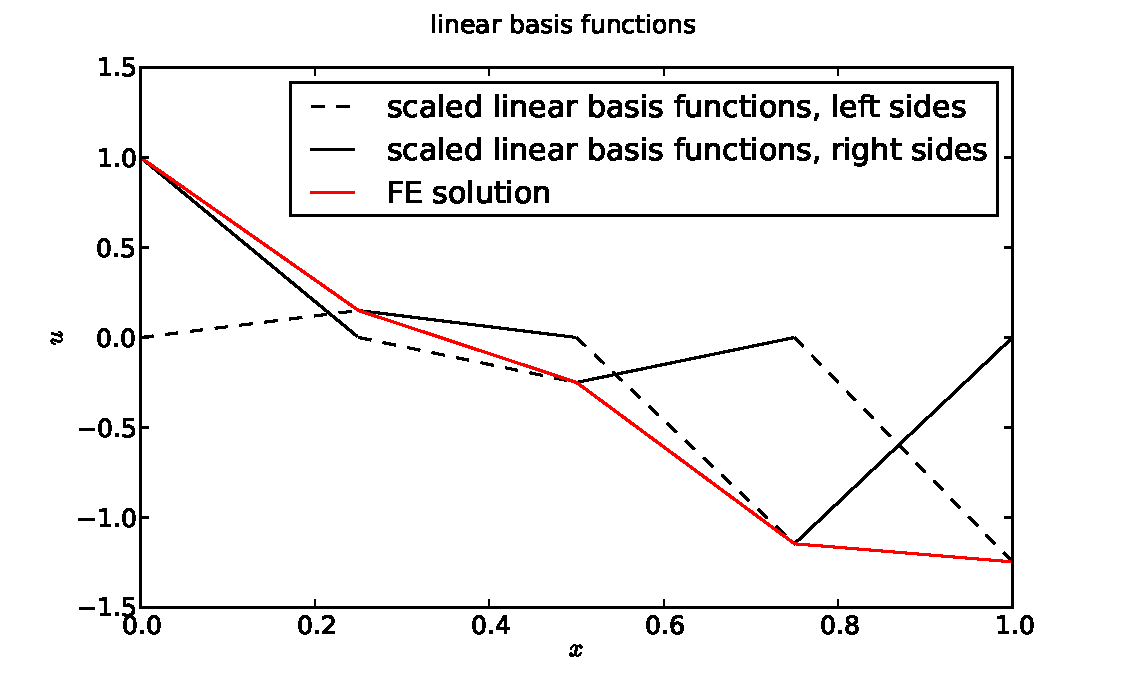
\includegraphics[width=\columnwidth,keepaspectratio=true]{./hw7-basis_functions-N5.pdf}
    % hw7-basis_functions-N5.pdf: 1000x600 pixel, 100dpi, 25.40x15.24 cm, bb=0 0 720 432
    \caption{Five basis functions.}
    \label{fig:N5}
\end{figure}

\begin{figure}[ht]
    \centering
    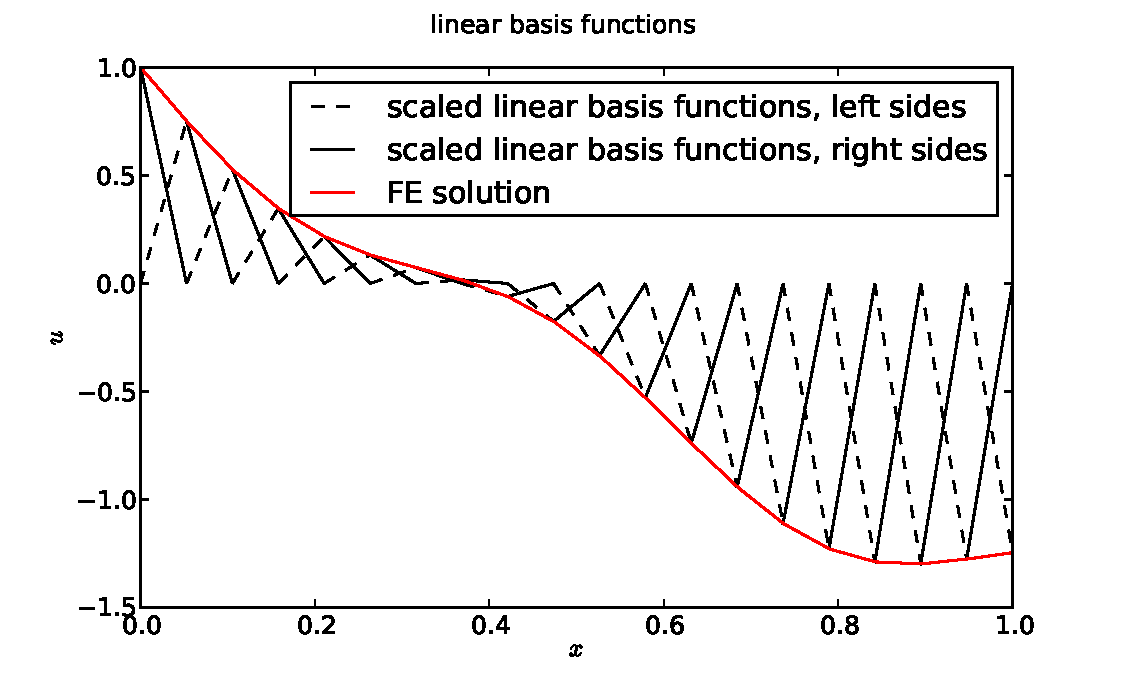
\includegraphics[width=\columnwidth,keepaspectratio=true]{./hw7-basis_functions-N20.pdf}
    % hw7-basis_functions-N20.pdf: 1000x600 pixel, 100dpi, 25.40x15.24 cm, bb=0 0 720 432
    \caption{Twenty basis functions.}
    \label{fig:N20}
\end{figure}

\begin{figure}[ht]
    \centering
    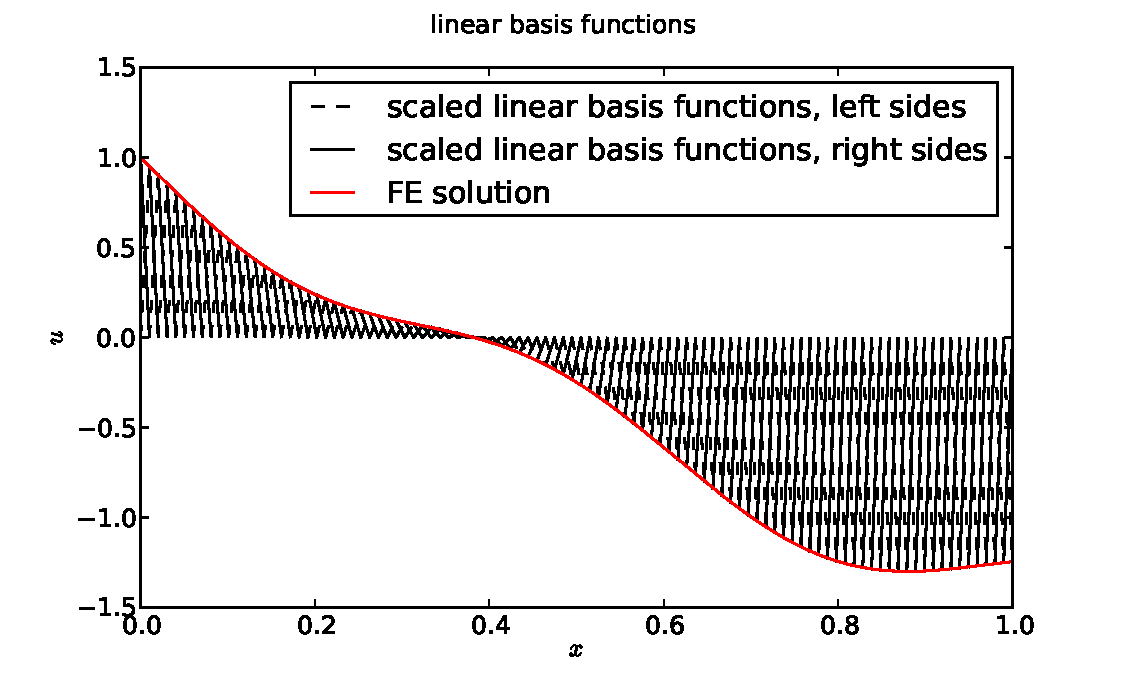
\includegraphics[width=\columnwidth,keepaspectratio=true]{./hw7-basis_functions-N100.pdf}
    % hw7-basis_functions-N100.pdf: 1000x600 pixel, 100dpi, 25.40x15.24 cm, bb=0 0 720 432
    \caption{One hundred basis functions.}
    \label{fig:N100}
\end{figure}

\begin{figure}[ht]
    \centering
    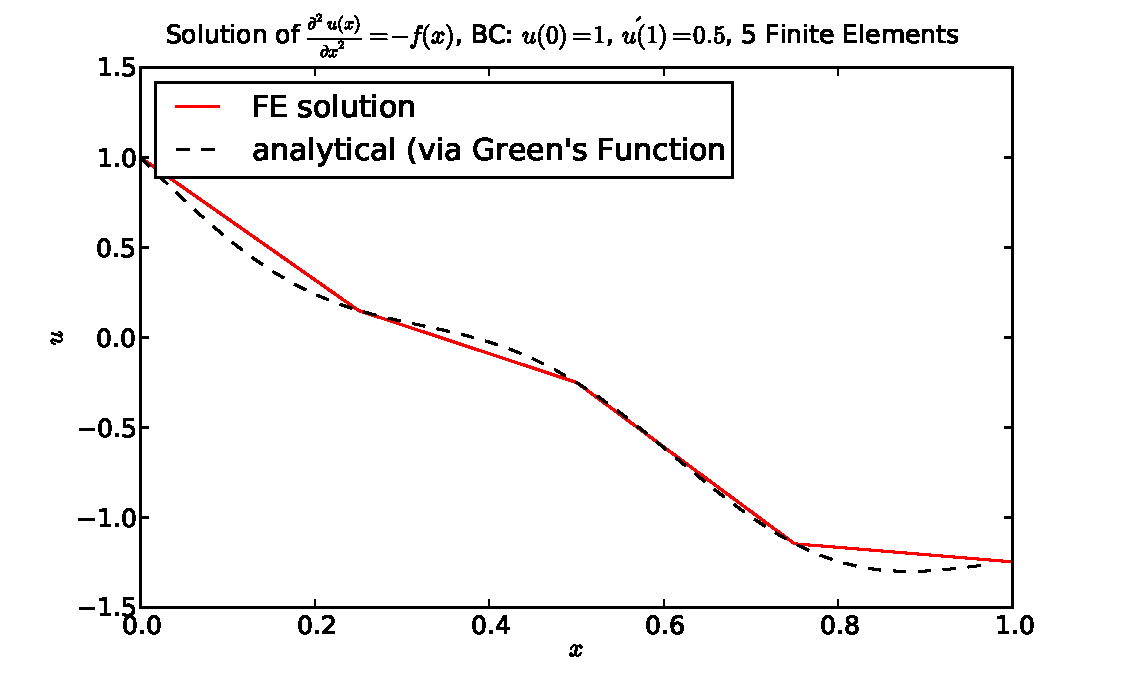
\includegraphics[width=\columnwidth,keepaspectratio=true]{./hw7-solution_and_forcing-N5.pdf}
    % hw7-solution_and_forcing-N5.pdf: 1000x600 pixel, 100dpi, 25.40x15.24 cm, bb=0 0 720 432
    \caption{Solution and forcing, 5 basis functions.}
    \label{fig:sf5}
\end{figure}

\begin{figure}[ht]
    \centering
    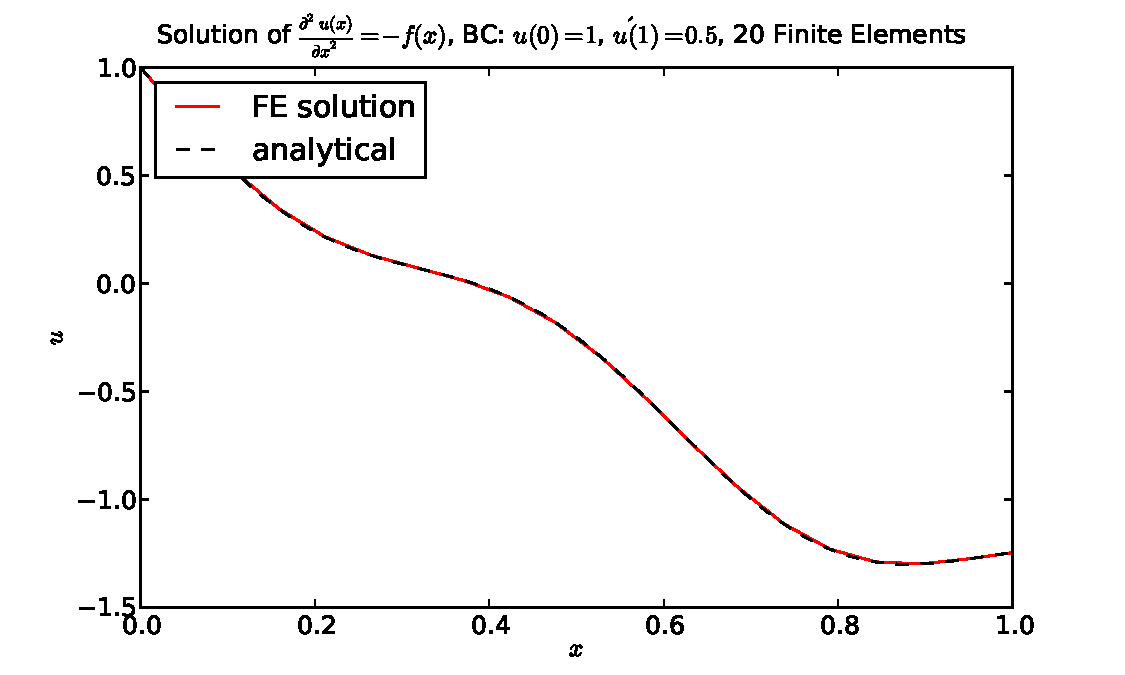
\includegraphics[width=\columnwidth,keepaspectratio=true]{./hw7-solution_and_forcing-N20.pdf}
    % hw7-solution_and_forcing-N5.pdf: 1000x600 pixel, 100dpi, 25.40x15.24 cm, bb=0 0 720 432
    \caption{Solution and forcing, 20 basis functions.}
    \label{fig:sf20}
\end{figure}

\begin{figure}[ht]
    \centering
    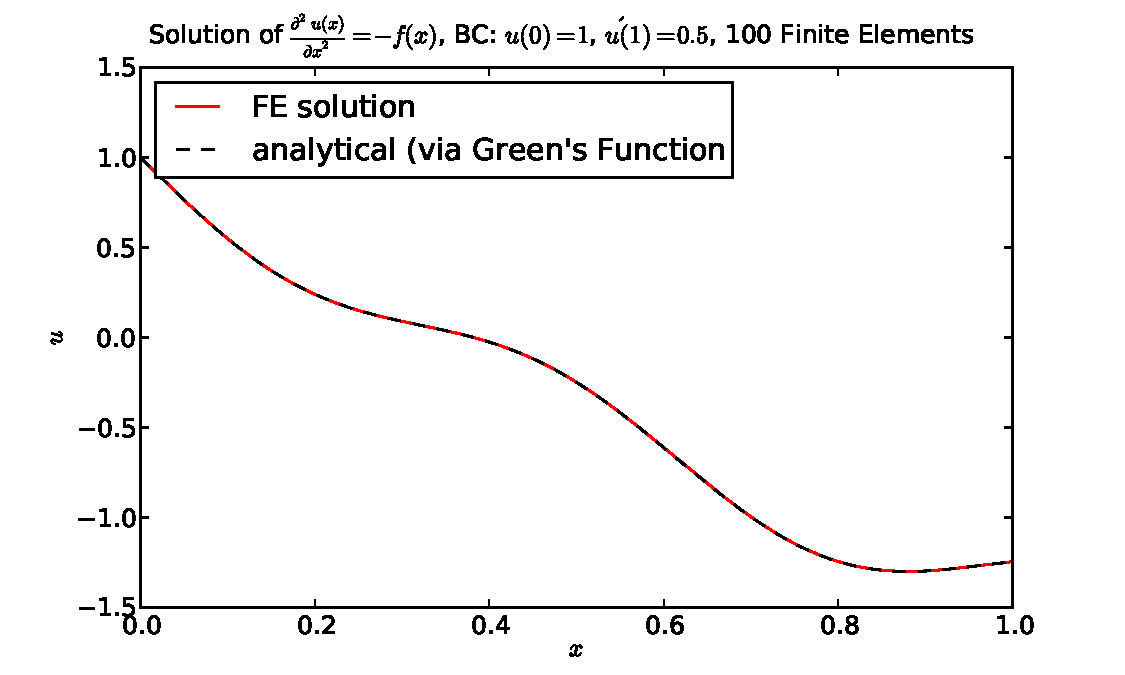
\includegraphics[width=\columnwidth,keepaspectratio=true]{./hw7-solution_and_forcing-N100.pdf}
    % hw7-solution_and_forcing-N5.pdf: 1000x600 pixel, 100dpi, 25.40x15.24 cm, bb=0 0 720 432
    \caption{Solution and forcing, 100 basis functions.}
    \label{fig:sf100}
\end{figure}

\begin{figure}[ht]
    \centering
    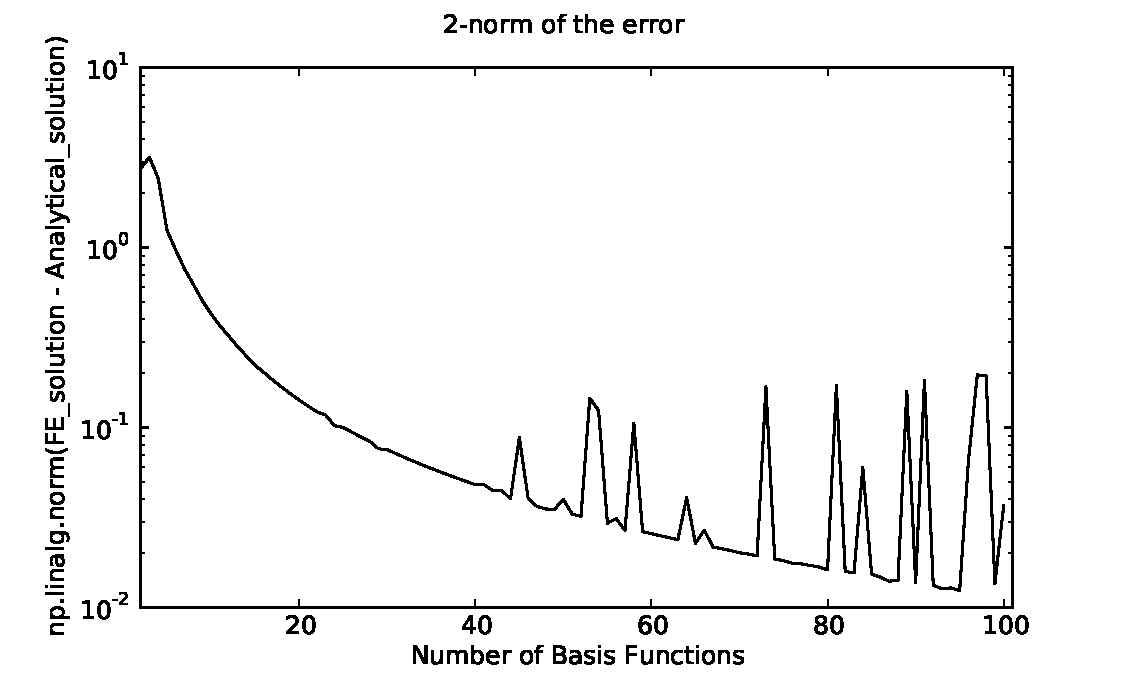
\includegraphics[width=\columnwidth,keepaspectratio=true]{./hw7-error_rate.pdf}
    % hw7-error_rate.pdf: 1000x600 pixel, 100dpi, 25.40x15.24 cm, bb=0 0 720 432
    \caption{Rate of error reduction with increasing number of basis functions (decreasing discretization distance).}
    \label{fig:errorrate}
\end{figure}

\clearpage

\section{Code}

\code{hw7.py}{hw7.py}

\end{document}          
